% Compile with: latexmk -pdfxe -outdir=build
\documentclass[12pt,oneside]{LuThesis}

\title{Saules paneļu efektivitāte Latvijas klimatā}
\author{Viktorija Leimane}

%%% LuThesis deklerācijas
\def\studaplnum{vl16047}
\def\darbvad{Dr. Phys. Andris Jakovičs}
\def\dokfak{\textbf{Fizikas, matemātikas un optometrijas fakultāte}}
\def\recenzents{Dr. Phys.Aivars Vembris}
\def\doktitle{\textbf{Saules paneļu efektivitāte Latvijas klimatā}}
\def\dokfak{\textbf{Fizikas, matemātikas un optometrijas fakultāte}}
\def\dokdate{} % Darba vadītāja parakstīšanas datums
\def\dokdateiesn{} % Darba iesniegšanas datums

%%% Valodas un fonti
\setdefaultlanguage{latvian}
\setotherlanguage{english}
\setmainfont[BoldFont=FreeSerifBold.ttf,ItalicFont=FreeSerifItalic.ttf,BoldItalicFont=FreeSerifBoldItalic.ttf]{FreeSerif.ttf}

\usepackage{graphicx}

%%% Misc
% \usepackage{hyperref}
\usepackage[hidelinks]{hyperref}
\addbibresource{bachelor.bib} % biblatex bibliotēkas fails: bachelor.bib
\usepackage[section]{placeins}
\usepackage[toc,page]{appendix}

%%% Dokumenta struktūra
\begin{document}

\maketitle

% * Anotācija
\chapter*{Anotācija}
\setcounter{page}{1}
\begin{abstract}
Darba mērķis ir noteikt efektīvāko saules paneļu izvietojuma veidu Latvijai tipiskos meteoroloģiskajos apstākļos. 
Balstoties uz divu veidu saules paneļiem, kas novietoti piecās dažādās telpiskajās orientācijās Latvijas Universitātes Botāniskā dārza teritorijā, tiks noteikta solāro paneļu efektivitātes atkarība no mainīgiem parametriem:
1) meteoroloģiskie apstākļi
2) telpiskā orientācija
3) gada mēnesis
4) solāro paneļu tips. \\
Iegūtie monitoringa rezultāti tiks analizēti kontekstā ar šo paneļu efektivitātes fizikālo novērtējumu.\\

\keywords{Saules enerģijas paneļi, atjaunojamo energoresursu enerģija, vides monitorings}
\end{abstract}

\chapter*{Abstract}
\begin{english}
\begin{abstract}
The aim of this thesis is to determine the most efficient way of solar panel arrangement for the climatic conditions of Latvia.
Based on two types of solar panels placed in five different spatial orientations in the University of Latvia Botanical Garden area, the dependency of the efficiency of solar panels on following variable parameters is established:
\begin{enumerate}
\item type of solar panels
\item spatial orientation
\item month of year
\item meteorological conditions.
\end{enumerate}

The results of the monitoring are analysed in the context of solar irradiance intensity, the physical assessment of the partial(?) efficiency of the panels and the results of other measurements.

\keywords{Solar panels, renewable energy}
\end{abstract}
\end{english}

%* Saturs
\tableofcontents

%* Apzīmējumu saraksts
\chapter*{Apzīmējumu saraksts}
\addcontentsline{toc}{chapter}{Apzīmējumu saraksts}
\noindent 
\textbf{Klimats}\\
TSI - Kopējais saules apstarojums, $\textrm{Wm}^{-2}$\\
SSI - Saules spektrālais apstarojums, $\textrm{Wm}^{-2}\textrm{nm}^{-1}$\\
% $G_{sc}$ - Solārā konstante, $\textrm{Wm}^{-2}$\\
%Photovoltaic power potential
TIM - Kopējā apstarojuma novērotājs\\
GHI – Globālais horizontālais apstarojums,  $\textrm{kWh/m}^2$\\ %Global horizontal irradiation
DHI – Difūzais horizontālais apstarojums,  $\textrm{kWh/m}^2$\\ 
DNI – Tiešais normālais apstarojums, $\textrm{kWh/m}^2$\\ %Direct normal irradiation
CMF - Mākoņu modifikācijas reizinātājs\\
AU - astronomiskā vienība\\  %astronomical unit
\textbf{Saules kustības leņķi}\\
$\theta$ - staru krišanas leņķis uz saules paneli\\
$\delta$ - Saules deklinācija -- leņķis starp virzieniem uz Sauli un debess ekvatoru solārajā pusdienlaikā.\\
 $\phi$  - ģeogrāfiskais platums; pozitīvs Z virzienā.\\
$\beta$  - paneļa slīpums -- leņķis starp Saules paneļa virsmu un horizontāli.\\
$\gamma$ - paneļa azimuts -- leņķis starp virsmas normāles projekciju uz horizontālo  plakni un D virzienu.\\
$\omega$ - solārais stundu leņķis -- leņķis starp Saules stara virziena projekciju uz horizontālo plakni un D virzienu; negatīvs no rīta.\\
\textbf{Saules paneļi}\\
PV - fotoelektriskais elements\\ %fotogalvanisks?
Si - silīcijs\\
P - jauda, 	W\\
Pmax - maksimālā jauda, W\\
PVOUT – Saules fotoelementa potenciālā jauda, $\textrm{kWh/kWp}$\\ 
%Photovoltaic power potential
E$_{norm}$, $\textrm{kWh/m}^2$ - enerģija normēta uz saules paneļa laukuma vienību.\\
\textbf{Debespuses}\\
A - austrumi\\
R - rietumi\\
D - dienvidi\\

%* Ievads
\chapter*{Ievads}
\addcontentsline{toc}{chapter}{Ievads}
Apvienoto Nāciju Organizācijas Klimata konferencē Parīzē 2015. gada decembrī daudzas pasaules valstis vienojās ierobežot globālo sasilšanu zem 2\textdegree C salīdzinājumā ar pirmsindustriālo laikmetu.
%, tāpēc ES ir apņēmusies līdz 2030. gadam samazināt siltumnīcefekta gāzu emisijas vismaz par 40\% salīdzinājumā ar 1990. gada līmeni.
Tāpēc Eiropas Savienībā noteikts dalībvalstīm saistošs mērķrādītājs  –  vismaz 32\%  atjaunojamās enerģijas īpatsvars līdz 2030. gadam \cite{ES}.

Ne mazāk būtiska ir atjaunojamo energoresursu loma energoapgādes neatkarības un drošības veicināšanā, tehnoloģiju attīstībā un inovācijās, vienlaikus sniedzot labumu videi un sabiedrībai, kā arī nodrošinot svarīgus priekšnosacījums nodarbinātībai, reģionālajai attīstībai un elektrības nodrošināšanai grūti pieejamās vietās \cite{ES}.

Dažādu atjaunojamo enerģijas resursu - saules, vēja, ģeotermālo un ūdens - starpā Saules enerģija ir viens no kandidātiem klimata pārmaiņu un to seku mazināšanai un efektīvas energoapgādes nodrošināšanai. Pēdējā desmitgadē veiktās investīcijas Saules enerģijas izmantošanā manifestējās inovācijās saules paneļu ražošanā, un gala rezultātā tie ir kļuvuši efektīvāki un finansiāli pieejamāki patērētājiem, piemēram, silīcija saules paneļu cena sastāda $\leq$ 30\% no kopējām saules paneļu sistēmas uzstādīšanas izmaksām un to saražotā enerģija atkarībā no atrašanās vietas un paneļa veida atmaksājas pēc $\geq$ 3 gadu perioda \cite{researchOpp}. Tomēr bez klimata to efektivitāti ietekmē arī daudzi citi faktori, kas tiek analizēti šajā darbā, piemēram, saules paneļu tips un telpiskā orientācija.

Šī pētījuma \textbf{mērķis} ir analizēt un praktiski pārbaudīt divu tipu (JA un LG) saules paneļu efektivitāti atšķirīgos telpiskās orientācijās risinājumos -- pētītas trīs dažādu virzienu (dienvidu (D), rietumu (R), austrumu (A)) un trīs leņķu pret horizontu (13\textdegree, 40\textdegree, 90\textdegree) paneļu grupas -- un tiek salīdzināta to piemērotība Latvijas klimatiskajiem apstākļiem.

% \subsection{Darba uzdevumi}
\textbf{Darba uzdevumi}
\begin{itemize}
\item Ievākt, atlasīt un analizēt saules paneļu jaudas (P) datus.
\item Izveidot iespējami automatizētu datu apstrādes sistēmu R valodā ilgtermiņa montioringa vajadzībām.
\item Salīdzināt paneļu efektivitāti gada laikā mēnešu intervālos atbilstoši tipa un telpiskās orientācijas apakšgrupām.
% \item Balstoties uz ilgtermiņa saules izstarojuma monitoringu, novērtēt saules paneļu saražoto enerģiju no fizikālajiem apsvērumiem.
\item Novērtēt datu kvalitāti no fizikālo apsvērumu un saules apstarojuma mērījumu viedokļa.
\end{itemize}

% \subsection{Darba aktualitāte}
\textbf{Darba aktualitāte}

Darba nozīme atklājas detalizētas paneļu efektivitātes analīzes nepieciešamībā tieši Latvijas klimatiskajiem apstākļiem. Latvijā veikto pētījumu daudzums un kvalitāte pagaidām neļauj iegūt pilnīgu priekšstatu par Saules paneļu lietošanas iespējām un prognozēt dažādu paneļu tipu efektivitāti reālā Latvijas klimatā. Tāpēc šī darba novitāte ietverta programmatūras izveidē, kas ļauj attēlot un apstrādāt Saules paneļu monitoringa datus, kas dos iespēju veikt turpmākus dziļākus pētījumus par dažādiem saules paneļu spēkstaciju pielietojuma aspektiem Latvijā.\\
% \subsection{Darba struktūra}

\textbf{Darba struktūra}

Darba pirmo daļu veido literatūrā pieejamo Saules apstarojuma novērtējumu raksturojums un apskats par Saules redzamo pārvietošanās pie debess sfēras diennakts laikā 60 dienu intervālos. Otrajā daļā aplūkota saules paneļu uzbūve un to darbības princips. Trešajā daļā tiek apskatīta saules paneļu sistēmas elektriskā shēma un raksturoti LU Botāniskā dārza spēkstacijas instalācijas parametri.
Ceturtajā daļā ir aprakstīti iegūtie rezultāti, tie ir salīdzināti savā starpā, ar citas saules paneļu spēkstacijas mērījumu rezultātiem, ar eksperimentālā poligona meteostacijas datiem par solāro apstarojumu šajā laika periodā, kā arī aplūkoti no teorētiskās pusvadītāju fizikas aspektiem.\\

\textbf{Autores ieguldījums darbā}
% \subsection{Autores ieguldījums darbā}
% the \\ insures the section title is centered below the phrase: Appendix B

Saules paneļu uzstādīšanu veica SIA EG Inženieri Valda Gailīša vadībā.
Par datu ievākšanu no saules paneļu sistēmas datu uzkrājējiem jāpateicas Victron Energy B.V. izstrādātājai VRM sistēmai.

Mans ieguldījums ir koda arhitektūras plānošana, rakstīšana un uzturēšana līdz šim brīdim. Esmu vienīgais koda bāzes izstrādātājs. Darbā kopā veikti 318 iesūtījumi (\textit{commits}) trīs zaros (105, 123 un 90 iesūtījumi attiecīgi), kas rezultējās 3140 koda rindās. 

Darba gaitā veicu datu lejupielādi, datu informācijas aptveršanu, kā arī datu programmatisku atlasīšanu, apstrādi, apkopošanu, transformēšanu vizualizācijas vajadzību pielāgošanai un datu vizualizāciju. 

% \begin{figure}[h]
% 	\centering
% 	\includegraphics[width=0.6\linewidth]{figures/misc/contributions.png}
% 	\caption{Darba autores ieguldījums master zarā.}
% 	\label{fig:retribution}
% \end{figure}
% % TEORIJAS KOPSAVILKUMS
Vispirms tiek aplūkota Saules emitētā starojuma daba un ģeometriskie apsvērumi - virziens, no kura staru kūlis sasniedz virsmu, leņķis uz virsmas un laika gaitā saņemtais starojuma daudzums. Tiek apskatīta atmosfēras un mākoņu ietekme uz virsmas saņemto saules starojumu, un tās praktiskā nozīme, apstrādājot pieejamos Saules starojuma datus, lai aprakstītu radiācijas gadījumus uz virsmas dažādās orientācijās.

% atjaunojamā enerģija
% kāpēc ir svarīgi
% 	politika (direktīva)
% 	klimata pārmaiņas
% atjaunojamās enerģijas veidi (vējš, saule, utml)
% mērķis ir salīdzināt solāro paneļu saražoto enerģiju atkarībā no modeļa, telpiskās orientācijas, leņķa un kā mainās pa gadalaikiem tieši latvijā
% citos klimatiskajos apstākļos līdzīgas analīzes ir veiktas ko var iegūt dažādās klimatiskajās zonās
% pierakstīt par pv paneļu darbību un efektivitāti
% aprakstīt ko tu darīji, lai pēc iespējas automatizētu datu apstrādes sistēmu
% kādus datus uzkrāj kādā attēlojumā
% datu menedžmentu aprakstīt
% paskatīties kā nosaka solāro paneļu efektivitātes standartu
% sarēķināt attiecības starp paneļu saražoto (normēt uz lielāko paneli)
% ielikt grafikus no februāra un aprīļa
% pierakstīt salīdzinājumu
% aprakstīt gļukus, kur dienā nav nekā saražots bet blakus ir. tā gadās.
% nomaini februāra sol_month grafikos virsrakstu uz februāri
% nomaini $Em^-2$ uz $E_norm$

% * Literatūras apskats
\chapter{Literatūras apskats}
% \section{Definīcijas}
Saules plankums - magnētiskās plūsmas koncentrācija bipolāros klāsteros vai grupās, kas novērojama kā tumšs plankums uz Saules fotosfēras.\\
Saules plankumu cikls - aptuveni 11 gadus ilga kvaziperiodiska variācija saules plankuma skaitlī. Magnētiskā lauka polaritātes modelis mainās ar katru ciklu.\\
Saules plankuma skaitlis - Dienas saules plankuma aktivitātes indekss (R), definēts kā R = k(10g + s), kur
s - individuālo plankumu skaits;
g - saules plankumu grupu skaits;
k - observatorijas faktors.
total solar irradiance (TSI) - Solar energy per unit time over a unit area perpendicular to the Sun’s rays at the top of Earth’s atmosphere.
% \\http://lasp.colorado.edu/home/sorce/reference/glossary/
\input{tex/literatura}
% intensity
% spectral distribution
% solar geometry
% saules stāvoklis debesīs
% un virziens, kurā stara starojums krīt uz dažādu virzienu un ēnojuma virsmām

\section{Saules apstarojums}

Lielākā daļa Saules emitētās enerģijas tiek saražota kodolreakcijās fotosfērā.

% Saņemto enerģiju laika vienībā uz uz laukuma vienības perpendikulāri starojuma izplatīšanās virzienam 1 AU attālumā integrēta pa visiem viļņu garumiem raksturo solārā konstante ($G_{sc}$).

Solārā konstante $G_{sc}$ ir saņemtā enerģija laika vienībā uz laukuma vienības perpendikulāri starojuma izplatīšanās virzienam 1 AU attālumā integrēta pa visiem viļņu garumiem.\cite{ThermalProcesses}

Kopējā saules apstarojuma vērtība mainās laikā un korelē ar Saules plankumu ciklu.
Viena fizikālā lieluma tikai daļēji pārklājušos novērojumu laikrindu apvienošana kompozītā ir gan zinātnisks, gan statistisks izaicinājums un neviens kompozīts (piemēram, PMOD, ACRIM, IRBM) līdz šim nav guvis konsensu solārā apstarojuma pētnieku kopienā.~\ref{fig:TSI_misijas}

Par labāko saules apstarojuma mērījumu reprezentāciju tiek uzskatīti TIM instrumenta dati mēraparāta uzbūves (TIM ir lielāka precizitātes apertūra tuvu dobumam un mazāka redzeslauku bloķējošā pie instrumenta ieejas, klasiskajos radiometros ir pretēji, kas palielina jutību pret atstaroto gaismu no redzeslauku bloķējošās apertūras un kļūdu no instrumenta sasildīšanas) un augstās precizitātes dēļ, tāpēc šajā darbā grafiki balstās uz šiem mērījumiem, pēc kuriem absolūtā kopējā saules apstarojuma vērtība ir $1360.8 \pm 0.5 \textrm{Wm}^{-2}$.\cite{Frohlich2012}

\begin{figure}[h]
    \centering
    \includegraphics[width=0.6\linewidth]{figures/misc/TSI_misijas.png}
    \caption{Salīdzinājums dienā vidējotiem saules kopējā apstarojuma datiem no dažādām misijām un Saules plankuma skaitlis, lai ilustrētu solārās aktivitātes variabilitāti trīs ciklos. \cite{Frohlich2012}}
    \label{fig:TSI_misijas}
\end{figure}

\begin{table}[h]
    \caption{TSI mērījumu vēsture} % caption iet pirms tabulas
    \begin{center}
    \begin{tabular}{| r | c | l |}
    \hline
    radiometrs & misija & darbības laiks \\ \hline
    Hickey-Frieden & NIMBUS-7 & 1978--1992  \\ \hline
	ACRIM I & Solārā Maksimuma Misija (SMM) & 1980--1989 \\ \hline
	ACRIM  & Zemes Radiācijas Budžeta Satelīts (ERBS) & 1984--2003 \\ \hline
	ACRIM II & Augšējās Atmosfēras Izpētes Satelīts (UARS) & 1991--2001 \\ \hline
	VIRGO & Solārā un Heliosfēras observatorija (SOHO)& 1996--pašlaik \\ \hline
	ACRIM III & ACRIMSAT  & 2000--pašlaik \\ \hline
	TIM & Saules Radiācijas un Klimata Eksperiments (SORCE) & 2003--pašlaik\\ \hline
    \end{tabular}
    \end{center}
    \label{tab:radiometers}
\end{table}


% Kopējais saules apstarojums (TSI) ir saules starojuma absolūtās intensitātes mērījums integrēts visā saules enerģijas diskā un visā saules enerģijas spektrā.
% diennakts vidējais apstarojums 1 AU attālumā no Saules.
% Norāda uz solārās radiācijas izmaiņām, kas ietekmē solārās enerģijas apjomu uz Zemes atmosfēras augšējiem slāņiem.


\begin{figure}[h]
    \centering
    \includegraphics[width=\linewidth]{figures/misc/TSI_8-19.pdf}
    \caption{Kopējais saules apstarojums 24. saules ciklā \cite{TSIdata}}
    \label{fig:TSI1}
\end{figure}

\begin{figure}[h]
    \centering
    \includegraphics[width=\linewidth]{figures/misc/TSI.pdf}
    \caption{Kopējais saules apstarojums solāro paneļu datu ieguves laikā \cite{TSIdata}}
    \label{fig:TSI2}
\end{figure}

\begin{figure}[h]
    \centering
    \includegraphics[width=\linewidth]{figures/misc/LV_DNI.png}
    \caption{Tiešais normālais apstarojums \cite{solargis}}
    \label{fig:lv_DNI}
\end{figure}
\begin{figure}[h]
    \centering
    \includegraphics[width=\linewidth]{figures/misc/LV_GHI.png}
    \caption{Globālais horizontālais apstarojums Latvijā \cite{solargis}}
    \label{fig:lv_GHI}
\end{figure}
\begin{figure}[h]
    \centering
    \includegraphics[width=\linewidth]{figures/misc/LV_PVOUT.png}
    \caption{PV potenciālā jauda \cite{solargis}}
    \label{fig:lv_PVOUT}
\end{figure}

% !TeX spellcheck = lv_LV
% intensity
% spectral distribution
% solar geometry
% saules stāvoklis debesīs
% un virziens, kurā stara starojums krīt uz dažādu virzienu un ēnojuma virsmām

\subsection{Saules stāvoklis debesīs}
Apzīmēsim ar $\theta$ staru krišanas leņķi uz Saules paneli, pieņemot, ka Saules panelis ir plakans un nekustīgs. Tad, pie nemainīgās starojuma intensitātes, paneļa saņemtā enerģija būs proporcionāla $\cos{\theta}$ (ja $\theta<90^\circ$) vai būs vienāda ar 0 (ja $\theta>90^\circ$, t.i. Saules stari krīt uz paneļa apakšējo virsmu). Saules diennakts kustība, gadalaiku cikls, ka arī Saules paneļa novietojums ir ievēroti izteiksmē, kas saskaņā ar [Solar\_Engineering\_of\_Thermal\_Processes.pdf] ļauj aprēķināt $\cos{\theta}$:
\begin{equation}
\label{eq:theta}
\begin{aligned}
	\cos{\theta} = {} & \sin{\delta} \sin{\phi} \cos{\beta} - \sin{\delta} \cos{\phi} \sin{\beta} \cos{\gamma} +                           \\
	                  & \cos{\delta} \cos{\phi} \cos{\beta} \cos{\omega} + \cos{\delta} \sin{\phi} \sin{\beta} \cos{\gamma} \cos{\omega} + \\
	                  & \cos{\delta} \sin{\beta} \sin{\gamma} \sin{\omega},
\end{aligned}
\end{equation}
kur lietoti leņķi, kas definēti \ref{tab:theta} tabulā. Saules deklināciju solārajā pusdienlaikā var aprēķināt pēc formulas
\begin{equation}
\label{eq:delta}
    \delta = 23 \sin \left( 360 \cdot \frac{284+n}{365} \right),
\end{equation}
kur $n$ ir dienas kārtas numurs gadā.

Ar vienādojumu \ref{eq:theta} un \ref{eq:delta} palīdzību ir iespējams aprēķināt $\cos{\theta}$ atkarības no laika, kas ir pirmais tuvinājums Saules apstarojuma izmaiņām dienas laikā.
% Parametru vērtības katram no darbā lietotajiem Saules paneļiem ir apkopotas \ref{tab:param}. tabulā.
% Lietojot šos parametrus, tika aprēķinātas $\cos{\theta}$ atkarības no laika diviem datumiem: 1. janvārim un 31. aprīlim, sk. \ref{fig:cos-theta}. attēlā. Var redzēt, ka modelis paredz būtiskākas vienkāršas sakarības. Piemēram, austrumu virzienā vērsts panelis "ieslēdzas" agrāk par rietumu virzienā vērstu paneli. Otrkārt, janvārī no D paneļiem visefektīvākais ir vertikālais, jo Saule atrodas zemu, savukārt aprīlī visefektīvākais ir 40$^\circ$ leņķis.

\begin{table}[h!]
	\caption{Leņķu, kas lietoti \ref{eq:theta} vienādojumā, definīcijas.}
	\begin{center}
		\begin{tabular}{|c|c|l|}
			\hline
			         &         apgabals         & definīcija                                                                 \\ \hline\hline
			$\theta$ &  $(0^\circ;180^\circ)$   & staru krišanas leņķis uz Saules paneli                                     \\ \hline
			$\delta$ &  $(-23^\circ;23^\circ)$  & Saules deklinācija --- leņķis starp virzieniem uz Sauli un uz debess       \\
			         &                          & ekvatoru solārajā pusdienlaikā, pozitīvs Z virzienā                        \\ \hline
			 $\phi$  &  $(-90^\circ;90^\circ)$  & ģeogrāfiskais platums, pozitīvs Z virzienā                                 \\ \hline
			$\beta$  &  $(0^\circ;180^\circ)$   & paneļa slīpums --- leņķis starp Saules paneļa virsmu un horizontāli        \\ \hline
			$\gamma$ & $(-180^\circ;180^\circ)$ & paneļa azimuts --- leņķis starp virsmas normāles projekciju uz horizontālu \\
			         &                          & plakni un D virzienu, negatīvs A virzienā                                  \\ \hline
			$\omega$ & $(-180^\circ;180^\circ)$ & solārais stundu leņķis --- leņķis starp Saules stara virziena projekciju   \\
			         &                          & uz horizontālu plakni un D virzienu (kas mainās Zemes rotācijas ap         \\
			         &                          & savu asi dēļ), negatīvs no rīta                                            \\ \hline
		\end{tabular}
	\end{center}
	\label{tab:theta}
\end{table}

% \begin{table}[h!]
% 	\caption{Darbā lietotajiem Saules paneļiem atbilstošās leņķisko parametru vērtības, grādos.}
% 	\begin{center}
% 		\begin{tabular}{|r|c|c|c|c|c|}
% 			\hline
% 			         & R.13 & A.13 &   D.13   & D.40 & D.90 \\ \hline\hline
% 			paneļa slīpums $\beta$  & \multicolumn{3}{c|}{13} &  40  &  90  \\ \hline
% 			paneļa azimuts $\gamma$ &  90  & -90  & \multicolumn{3}{c|}{0}  \\ \hline
% 			ģeogrāfiskais platums $\phi$  &        \multicolumn{5}{c|}{57}        \\ \hline
% 		\end{tabular}
% 	\end{center}
% 	\label{tab:param}
% \end{table}

% \begin{figure}[h]
% 	\centering
% 	\includegraphics[width=\linewidth]{figures/misc/cos-theta-jan.pdf}
% 	\includegraphics[width=\linewidth]{figures/misc/cos-theta-apr.pdf}
% 	\caption{Diennakts laikā paredzētas $\cos(\theta)$ vērtības darbā lietotajiem Saules paneļiem, aprēķinātas pēc \ref{eq:theta} izteiksmes 1. janvārim (augšā) un 30. aprīlim (apakšā).}
% 	\label{fig:cos-theta}
% \end{figure}
% !TeX spellcheck = lv_LV
\section{Klimats Latvijā}
%Enter antagonists. Mākoņi. Bloķē daudz saules apstarojuma. Cik LV mākoņainu dienu?
%Izanalizēt VTPMML meteo datus no 2013.
%Pajautāt Stasim kļūdas.

Saskaņā ar LU VTPMML klimatisko datu apkopojumu, kas parādīts \ref{fig:makoni_Riga}. att., mākoņainība Rīgā var sasniegt līdz 60\% jūlijā un līdz pat 90\% decembrī. Tas nozīmē, ka Saules paneļu efektivitātes novērtējumam Latvijas klimatā ir jāņem vērā mākoņainība. Tas palīdzēs prognozēt nepieciešamus enerģijas uzkrājumus un papildavotus, ja solārā enerģija tiek izmantota kā pamata enerģijas avots.
\begin{figure}[h]
	\centering
	\includegraphics[width=0.8\linewidth]{figures/misc/makoni_riga.jpg}
	\caption{Vidējā mākoņainība Rīgā gada laikā, vidējota pa 20 gadu periodu. Attēls no [http://www.modlab.lv/klimats/Parametri/cloud/Cloud.html].}
	\label{fig:makoni_Riga}
\end{figure}

% Mākoņu ietekme uz Saules apstarojumu ir sarežģīta un atkarīga no vairākiem parametriem. Piemēram, G.~Pfistera pētījumā [cloud\_coverage\_impact\_on\_solar\_irradiance,pdf] tiek parādīts, ka dažreiz mākoņainība var pat nedaudz palielināt Saules apstarojumu. Šis šķietami paradoksālais rezultāts izskaidrojams ar to, ka Saule ar noteiktu varbūtību tomēr nav aizsegta, bet balti mākoņi var būt gaišāki, nekā pašas debesis saulainajā dienā (sk. \ref{fig:makoni_ietekme}.(b) attēlā). Tādā veidā DNI komponentes samazināšanās tiek kompensēta ar palielinātu gaismas izkliedi. Savukārt gadījumos, kad mākoņi aizsedz Sauli (sk. \ref{fig:makoni_ietekme}.(c) attēlā), apstarojums $\approx99\%$ gadījumu samazinās, kā tas bija paredzams. Tomēr korelācija starp iegūto enerģiju un mākoņu daudzumu ir pat nedaudz pozitīva, kas atkal notiek palielinātas gaismas izkliedes dēļ. Apskatot visu datu kopu, var secināt, ka vairākumā gadījumu mākoņu ietekmi uz Saules paneļu saražoto enerģiju var uzskatīt par nelabvēlīgu. Tomēr pētījuma autori norāda, ka, neskatoties uz to, ka mākoņainība ir galvenais Saules paneļu efektivitāti ietekmējošs faktors, informācija tikai par mākoņainību nav pietiekama, lai izskaidrotu un paredzētu paneļu saražotās enerģijas izmaiņas. Tas notiek arī tad, ja ņem vērā, vai Saule ir aizsegta ar mākoņiem.
\begin{figure}[h]
	\centering
	\includegraphics[width=\linewidth]{figures/misc/makoni_ietekme.jpg}
	\caption{Attiecība starp izmērīto apstarojumu un tīrās debess gadījuma apstarojumu (a) visiem datiem, (b) gadījumos ar neaizsegtu Sauli un (c) gadījumos ar aizsegtu Sauli. Attēls no [cloud\_coverage\_impact\_on\_solar\_irradiance,pdf].}
	\label{fig:makoni_ietekme}
\end{figure}

Mākoņu ietekme ir atkarīga arī no to veida. Lielums CMF (angl. \textit{Cloud Modification Factor}, mākoņu modifikācijas reizinātājs), ko definē kā attiecību starp apstarojumu gadījumos ar un bez mākoņiem, atkarībā no mākoņu tipa ir apkopots \ref{tab:CMF}. tabulā. Ir jāņem vērā, ka CMF ir atkarīgs no viļņa garuma. Tomēr ultravioletais CMF no redzamās gaismas CMF ir atkarīgs lineāri ar koeficientiem $\approx0.6-1$ gubumākoņu gadījumā un eksponenciāli spalvmākoņu gadījumā.
\begin{table}[h]
	\caption{CMF intervāls atkarībā no mākoņu tipa[effect\_of\_clouds\_on\_surface\_ubv.pdf]}
	\begin{center}
		\begin{tabular}{| r | c |}
			\hline
			augstie gubumākoņi & $<0.7$     \\ \hline
			gubumākoņi         & $0.2-1.3$ \\ \hline
			spalvmākoņi        & $0.6-1$    \\ \hline
		\end{tabular}
	\end{center}
	\label{tab:CMF}
\end{table}

Mākoņu ietekmes uz Saules apstarojumu modelēšana ir ļoti sarežģīta. Mērījumi parāda, ka mākoņi absorbē par 25 W/m$^2$ vairāk gaismas, nekā teorētiski paredzams, un šī vērtība nevar būt izskaidrojama ar troposfēras aerosoliem
% [absorbtion\_of\_solar\_radiation\_by\_cloouds.pdf].
% Sekmīgajai modeļa darbībai ir nepieciešama parametru verifikācija, ko ir grūti veikt mazāk attīstītās valstīs, kur eksperimentālo datu skaits nav tik izsmeļošs, kā attīstītajās valstīs. Šādos apstākļos statistiska pieeja (piemēram, iepriekš iegūto klimatisko datu vidējošana un ekstrapolēšana) var izrādīties vienkāršāka un dažreiz pat precīzāka par matemātiskajiem modeļiem [shorturl.at/mDNT3]. Papildus grūtības rada arī tas, ka Saules apstarojums svārstās Saules aktivitātes ciklu dēļ. Tomēr šā darba ietvaros to var neņemt vērā salīdzinoši nelielas ietekmes dēļ, jo GHI mainās tikai ap 0.7~W/m$^2$ gadā
% [changes\_of\_solar\_radiation\_at\_earth\_surface.pdf].
\section{Saules paneļi}
% KĀ STRĀDĀ SAULES PANEĻI?
% fotons uzspīd elektronam un viņu ierosina un tad tas aiziet pāri vadītspējas zonai un aizpeld uz elektrodu un caurums aizpeld uz otru elektrodu un rodas potenciālu starpība no kurienes strāva.
% Ielikt dokus par LG un JA tipu + no kādiem kristāliem tie
% Ielikt shēmu
% analīze par saules paneļu plantācijām pasaulē
% optimālie apstākļi?

Saules paneļi sastāv no fotoelementiem, kas pārveido gaismas enerģiju elektriskajā enerģijā. Fotoelements, kura struktūras shēma ir parādīta \ref{fig:PV}. attēlā, ir p-n pāreja ar elektriskiem kontaktiem, kas pieslēgti pie lādētāja vai citas enerģijas patērētāja. Fotoelementa apakšējā daļa sastāv no n-tipa pusvadītāja, kurā lādiņa pamatnesēji ir elektroni, bet augšējā daļa --- no p-tipa pusvadītāja, kur lādiņa pamatnesēji ir caurumi. 

Fotoelementa darbība balstās uz iekšējo fotoelektrisko efektu --- parādību, kad elektrons tiek ierosināts ar gaismas kvantu un pāriet no valences zonas uz vadītspējas zonu. Kad tas notiek augšējā slānī (p-tipa pusvadītājā), elektrons atgrūžas no robežas starp slāņiem, kura ir negatīvi lādēta rekombinācijas dēļ. Negatīvi lādēta (no p-tipa pusvadītāja puses) robeža rada potenciālu starpību, kas veicina elektronu kustību pa vadiem uz patērētāju, tādā veidā radot elektrisko strāvu.

\begin{figure}[h]
    \centering
    \includegraphics[width=0.6\linewidth]{figures/misc/solar_cell.pdf}
    \caption{Saules paneļa shēma. Tas sastāv no fotoelementiem, kuru augšējais slānis veidots no p-tipa pusvadītāja, bet apakšējais --- no n-tipa pusvadītāja.}
    \label{fig:PV}
\end{figure}

P-tipa un n-tipa pusvadītāja īpašības var panākt, piemēram, dopējot silīcija kristālu ar attiecīgi III vai V grupas elementiem. Ja silīcija kristālam pievieno bora atomus nelielā koncentrācijā, izveidojas \ref{fig:p-n-type}. att. pa kreisi redzamā situācija. Katram Si atomam ir četri elektroni ārējā čaulā, ar kuru palīdzību atoms izveido četras kovalentās saites ar četriem citiem atomiem. Savukārt bors, būdams III grupas elements, var izveidot tikai trīs saites. Tādā veidā pie bora atoma parādās "caurums" --- nenoslēgta kovalentā saite, kas attēlā apzīmēta ar sarkanu līniju. Uz šo vietu var pārvietoties kāds no blakus esošiem elektroniem, bet tad neaizpildīta vieta parādīsies pie blakus esošā atoma. Tādā veidā var uzskatīt, ka caurums "pārvietojas", un nosaukt to par pozitīvo lādiņa nesēju. Šādus pusvadītājus sauc par p-tipa pusvadītājiem.

Ja silīcija kristālam pievieno fosfora atomus, izveidojas pretēja situācija --- pie P atoma parādās elektrons, kas nepiedalās saites veidošanā (sk. att. \ref{fig:p-n-type}., pa labi). Lai pārvietotos, brīvajam elektronam ir nepieciešams mazāk enerģijas nekā elektroniem, kas veido kovalentās saites starp Si atomiem. Tātad, lādiņa pamatnesēji n-tipa pusvadītājos ir elektroni, un šādus pusvadītājus sauc par p-tipa pusvadītājiem.

Dopējot divus blakus esošus Si kristāla apgabalus dažādā veidā, iegūst p-n pāreju. Uz robežas starp apgabaliem elektroni no n-tipa apgabala var difūzijas ceļā nokļūt uz p-tipa apgabalu un aizpildīt tos caurumus, kas atrodas pietiekami tuvu. To sauc arī par elektronu-caurumu rekombināciju. Tādā veidā p-tipa pusvadītāja mala uzlādējās negatīvi. 

\begin{figure}[h]
	\centering
	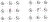
\includegraphics[width=0.5\linewidth]{figures/misc/p_n_type.pdf}
	\caption{Silīcija kristāla 2D izklājums, atomu ārējās čaulas elektroni ir apzīmēti ar punktiem. Pievienojot bora atomu, iegūst p-tipa pusvadītāju (pa kreisi), bet fosfora atomu --- n-tipa pusvadītāju (pa labi).}
	\label{fig:p-n-type}
\end{figure}
% otrā nodaļa - saules paneļu uzstādījums LU BD - shēma, utml

%* Rezultāti
\chapter{Rezultāti}
\input{tex/rezultati}
\section{Saules apstarojums}
% \begin{figure}[h]
%     \centering
%     \includegraphics[width=\linewidth]{figures/meteo/statsYears.pdf}
%     \caption{Solārā apstarojuma laika integrāļa atšķirības gada gaitā. Eksperimentālā poligona meteostacijas stacijas dati 2013 -- 2019 periodā.}
%     \label{fig:metYears}
% \end{figure}

% izlabo visur lu meteoroloģiju uz poligonu
% pārsaukt grafikā Em^-2 uz E_{norm} (normētais enerģijas blīvums)

Tieši ilgtermiņa saules apstarojuma monitorings saules paneļu uzstādīšanas vietā ir svarīgs paneļu efektivitātes prognozēšanas rīks, jo ļauj samazināt anomālu saulaina laika periodu svaru, kādi, piemēram, ir 2014. un 2019. gada aprīļi (skat. \ref{fig:metYears_mean}. att.). PV sistēmas veiktspējas monitoringam lietots Saules apstarojuma sensors (piranometrs), kas atrodas eksperimentālā poligona teritorijā. Šī mērierīce saules apstarojumu uztver ar plaknes virsmu no 180\textdegree skata leņķa, ko sauc par puslodes saules apstarojumu, un tās kļūda ir  $\pm 1 \%$ ~\cite{pyranometer}.

Attēlos \ref{fig:met_Irrad} un \ref{fig:met_Irrad_mean} redzams gaišo diennakts stundu momentānā saules apstarojuma integrāļi 5 minūšu intervālos novēroto četru mēnešu laikā, kas izskaidro turpmāk minētās atšķirības paneļu ražīgumā atkarībā no mēneša -- palielinās gan Saules spīdēšanas ilgums dienā (x ass), gan saņemtās enerģijas daudzums (y ass).

\begin{figure}[h]
    \centering
    \includegraphics[width=\linewidth]{figures/meteo/meanYears.pdf}
    \caption{Solārā apstarojuma laika integrāļa atšķirības gada gaitā un to vidējās vērtības. Eksperimentālā poligona meteostacijas stacijas dati 2013 -- 2019 periodā.}
    \label{fig:metYears_mean}
\end{figure}
\begin{figure}[h]
    \centering
    \includegraphics[width=\linewidth]{figures/meteo/sun19.pdf}
    \caption{Solārā apstarojuma izmaiņas dienas gaitā. Eksperimentālā poligona meteostacijas stacijas dati 2019-01-01 -- 2019-04-31 periodā.}
    \label{fig:met_Irrad}
\end{figure}
\begin{figure}[h]
    \centering
    \includegraphics[width=\linewidth]{figures/meteo/mean19.pdf}
    \caption{Mēnesī vidējotas solārā apstarojuma izmaiņas dienas gaitā. Eksperimentālā poligona meteostacijas stacijas dati 2019-01-01 -- 2019-04-31 periodā.}
    \label{fig:met_Irrad_mean}
\end{figure}
\section{Efektivitātes atkarība no parametriem}
\subsection{Saules paneļa tipa} \label{subsection:tipi}

Pēc tabulām \ref{tab:JA} un \ref{tab:LG}, kā arī grafikiem, kas ietverti diskusijā par citu parametru ietekmi uz efektivitāti (skat. \ref{subsection:gads}. nod.), redzams, ka LG tipa paneļi konsekventi ir efektīvāki par JA tipu. Tas ir saistīts gan ar kristāla veidu -- kā parādīts \ref{section:tipi}. nod.,  monokristāliska Si paneļi ir ražīgāki par polikristāliem --, gan paneļu maksimālajām jaudām -- LG
ir lielāka nominālā jauda uz laukuma vienību nekā JA.

\begin{table}[!htbp]
    \caption{JA tipa paneļu saražotā enerģija uz kvadrātmetru salīdzināta ar\\ enerģijas plūsmas blūvumu uz horizontālu virsmu}
    \begin{center}
    %%%%%%%%%%%%%%%%%%%%%%%%%%%%%%%%%%%%%%%%%%%%%%%%%%%%%%%%%%%%%%%%%%%%%%
%%                                                                  %%
%%  This is a LaTeX2e table fragment exported from Gnumeric.        %%
%%                                                                  %%
%%%%%%%%%%%%%%%%%%%%%%%%%%%%%%%%%%%%%%%%%%%%%%%%%%%%%%%%%%%%%%%%%%%%%%
\begin{tabular}{ | c | r r r r r  r | } \hline
E, $\textrm{kWhm}^{-2}$	&A.13	&R.13	&D.13	&D.40	&D.90	&piranometrs\\ \hline
jan		&0.35	&0.23	&0.72	&2.46	&2.80		&12.14\\
feb		&3.20	&2.74	&4.27	&6.45	&5.99		&25.14\\
mar		&8.22	&7.40	&9.47	&11.94	&8.72		&61.76\\
apr		&19.89	&19.23	&23.27	&25.43	&18.25		&141.41\\ \hline
$E_{sum}$, $\textrm{kWhm}^{-2}$
		&31.7	&29.6	&37.7	&46.3	&35.8 	&240.5\\ \hline
\end{tabular}
    \end{center} \label{tab:JA}
\end{table}
\begin{table}[!htbp]
    \caption{LG tipa paneļu saražotā enerģija uz kvadrātmetru salīdzināta ar\\ enerģijas plūsmas blūvumu uz horizontālu virsmu}
    \begin{center}
    %%%%%%%%%%%%%%%%%%%%%%%%%%%%%%%%%%%%%%%%%%%%%%%%%%%%%%%%%%%%%%%%%%%%%%
%%                                                                  %%
%%  This is a LaTeX2e table fragment exported from Gnumeric.        %%
%%                                                                  %%
%%%%%%%%%%%%%%%%%%%%%%%%%%%%%%%%%%%%%%%%%%%%%%%%%%%%%%%%%%%%%%%%%%%%%%
\begin{tabular}{ | c | r r r r r  r | } \hline
E, $\textrm{kWhm}^{-2}$	&A.13	&R.13	&D.13	&D.40	&D.90 	&piranometrs\\ \hline
jan	&0.5	&0.35	&0.95	&2.82	&3.22		&12.14	\\
feb	&4.43	&3.63	&5.05	&8.25	&7.41		&25.14	\\
mar	&10.92	&9.27	&11.27	&15.69	&11.34		&61.76	\\
apr	&27.63	&25.46	&29.14	&34.21	&23.18		&141.41	\\ \hline
$E_{sum}$, $\textrm{kWhm}^{-2}$
	&43.48	&38.7	&46.41	&60.98	&45.14		&240.46	\\ \hline
\end{tabular}
    \end{center} \label{tab:LG}
\end{table}

% %%%%%%%%%
\subsection{Saules paneļa leņķa}\label{subsection:degree}
Apkopojot četru mēnešu datus un abus paneļu tipus, visražīgākais leņķis ir 40\textdegree ~(skat.~\ref{fig:lg_ja_deg}. att.).
Kopumā var secināt, ka pret D orientētais panelis 90\textdegree ~leņķī saražo vairāk enerģijas ziemas mēnešos un 13\textdegree ~leņķī -- vasaras mēnešos, tātad apstiprinās teorijā (\ref{section:kustiba}.nod.) prognozētais.
% Tas sakrīt ar [ielikt grafiku ar LV karti un optimālo leņķi bet es neatceros no kurienes paņēmu to].
\begin{figure}[h!]
    \centering
    \includegraphics[width=\linewidth]{figures/results/all_degType.pdf}
    \caption{D virzienā vērsto saules paneļu saražotā enerģija atkarībā no leņķa un saules paneļu tipa} \label{fig:lg_ja_deg}
\end{figure}


\subsection{Saules paneļa virziena}\label{subsection:dir}
Visražīgākais virziens ir D, tad A, tad R (skat.~\ref{fig:lg_ja_dir}. att.). To paskaidro \ref{subsection:month_day}. nod. redzamie paneļu saražotās enerģijas dienas sadalījumi.
\begin{figure}[h!]
    \centering
    \includegraphics[width=\linewidth]{figures/results/all_dirType.pdf}
    \caption{13 grādu leņķī vērsto saules paneļu atkarība no virziena un saules paneļu tipa}
    \label{fig:lg_ja_dir}
\end{figure}

\subsection{Saules paneļa leņķa un virziena kombinācijas}
\label{subsection:month_day}

Saules paneļu saņemtā apstarojuma dienas sadalījuma tendenci drīkst salīdzināt ar attiecīgo paneļu saražotās enerģijas tendenci, jo pēdējā ir atkarīga no paneļa virsmas saņemtā Saules apstarojuma, kas savukārt ir funkcija no $cos(\theta)$, tātad proporcionāla tam. Salīdzinot \ref{fig:cos-theta}.(c) ar 
\ref{fig:toldU}, tiek secināts, ka eksperimentālie rezultāti sakrīt ar teoriju.

\begin{figure}[h]
    \centering
    \includegraphics[width=\linewidth]{figures/sol_day/apr_LG_13.pdf}
    \includegraphics[width=\linewidth]{figures/sol_day/apr_LG_D.pdf}
    \caption{Saules paneļu saražotās enerģijas dienas sadalījuma līkne vidējotiem 27-30. aprīļa datiem} \label{fig:toldU}
\end{figure}

Turpmāk apskatīts Saules apstarojuma dienas sadalījums mēnešos. Kā redzams \ref{fig:mar_ar}, \ref{fig:apr_ar}. att., eksperimentāli noteiktais saules paneļu saražotās enerģijas dienas sadalījums sakrīt ar teorētiski prognozēto \ref{fig:cos-theta}. att. kā arī labi novērojamas tā diennakts svārstības 30 dienu laikā.
% \begin{figure}[h]
%     \centering
%     \includegraphics[width=\linewidth]{figures/sol_day/feb_A13JA.pdf}
%     \includegraphics[width=\linewidth]{figures/sol_day/feb_R13JA.pdf}
%     \caption{A un R virzienu saules paneļu 5 minūtēs vidējotu Wh dienas sadalījumi februārī}
%     \label{fig:feb_ar}
% \end{figure}

\begin{figure}[h]
    \centering
    \includegraphics[width=\linewidth]{figures/sol_day/mar_A13JA.pdf}
    \includegraphics[width=\linewidth]{figures/sol_day/mar_R13JA.pdf}
    \caption{A un R virzienu saules paneļu 5 min intervālos integrētu jaudu dienas sadalījumi martā}
    \label{fig:mar_ar}
\end{figure}

\begin{figure}[h]
    \centering
    \includegraphics[width=\linewidth]{figures/sol_day/apr_A13JA.pdf}
    \includegraphics[width=\linewidth]{figures/sol_day/apr_R13JA.pdf}
    \caption{A un R virzienu saules paneļu 5 minūtēs vidējotu Wh dienas sadalījumi aprīlī}
    \label{fig:apr_ar}
\end{figure}

% % \begin{figure}[h]
% %     \centering
% %     \includegraphics[width=\linewidth]{figures/sol_month/feb_Dir_d.pdf}
% %     \includegraphics[width=\linewidth]{figures/sol_month/feb_Deg_d.pdf}
% %     \caption{Saules paneļu saražotā enerģija atkarībā no virziena un leņķa februārī}
% %     \label{fig:feb_degDir}
% % \end{figure}

% % \begin{figure}[h]
% %     \centering
% %     \includegraphics[width=\linewidth]{figures/sol_month/mar_Dir_d.pdf}
% %     \includegraphics[width=\linewidth]{figures/sol_month/mar_Deg_d.pdf}
% %     \caption{Saules paneļu saražotā enerģija atkarībā no virziena un leņķa martā}
% %     \label{fig:mar_degDir}
% % \end{figure}

% % \begin{figure}[h]
% %     \centering
% %     \includegraphics[width=\linewidth]{figures/sol_month/apr_Dir_d.pdf}
% %     \includegraphics[width=\linewidth]{figures/sol_month/apr_Deg_d.pdf}
% %     \caption{Saules paneļu saražotā enerģija atkarībā no virziena un leņķa aprīlī}
% %     \label{fig:apr_degDir}
% % \end{figure}

\subsection{Gada mēneša} \label{subsection:gads}
Pēc \ref{fig:jan_sum}, \ref{fig:feb_sum}, \ref{fig:mar_sum}, \ref{fig:apr_sum}. att., tiek izdarīti secinājumi par saules paneļu ražīguma atkarību no gada mēneša. Janvārī visefektīvākais panelis ir D.90, kas atbilst janvārim raksturīgajam Saules pārvietojumam -- zemu pie horzionta. \ref{fig:feb_sum}. att. redzams, ka februārī D.40 kļūst ražīgāks nekā D.90, tāpat redzams, ka mazāku leņķu paneļi -- R.13 un A.13 -- proporcionali vairāk Saules apstarojuma ir pārvērtuši enerģijā. Šī tendence novērojama arī turpmākajos mēnešos. Savukārt jau aprīlī visefektīvākā orientācija ir D.40. Visu telpisko orientāciju paneļi ir pakļauti Saules diennakts pārvietojuma izmaiņas izraisītajiem efektiem uz saražotās enerģijas apjomu, kas teorētiski aprēķināti \ref{section:kustiba}. nod.

% Janvārī visefektīvākaie ir paneļi, kas orientēti uz dienvidiem un novietoti vertikāli (D.90), jo Saule pārvietojas zemu gar horizontu. Savukārt jau aprīlī visefektīvākā orientācija ir D.40, un arī citu orientāciju paneļi ir pakļaut līdzīgiem efektiem, kas teorētiski aprēķināti \ref{section:kustiba}. nod.

Arī Ulbrokas saules paneļu spēkstacijas darbības analīze gada griezumā (skat. \ref{fig:ulbroka}. att.) uzrāda ļoti būtisku saules paneļu saražotās enerģijas variabilitāti gada mēnešos. Maksimālais enerģijas daudzums tiek saražots maijā, nedaudz mazāk citos vasaras mēnešos, bet janvārī, februārī, novembrī un decembrī saražotās enerģijas daudzums ir ļoti mazs. Šis apsvērums ir īpaši svarīgs industrializētos pielietojumos, jo ziemas mēnešos jādomā par alternatīvu enerģijas avotu.

\begin{figure}[h]
    \centering
    \includegraphics[width=\linewidth]{figures/sol_month/jan_m_m2.pdf}
    \caption{Saules paneļu saražotā enerģija janvārī}
    \label{fig:jan_sum}
\end{figure}

\begin{figure}[h]
    \centering
    \includegraphics[width=\linewidth]{figures/sol_month/feb_m_m2.pdf}
    \caption{Saules paneļu saražotā enerģija februārī}
    \label{fig:feb_sum}
\end{figure}

\begin{figure}[h]
    \centering
    \includegraphics[width=\linewidth]{figures/sol_month/mar_m_m2.pdf}
    \caption{Saules paneļu saražotā enerģija martā}
    \label{fig:mar_sum}
\end{figure}

\begin{figure}[h]
    \centering
    \includegraphics[width=\linewidth]{figures/sol_month/apr_m_m2.pdf}
    \caption{Saules paneļu saražotā enerģija aprīlī}
    \label{fig:apr_sum}
\end{figure}


\section{Salīdzinošā analīze}\label{section:effectivity}

Eksperimentāli noteiktā paneļu efektivitāte (skat.~\ref{tab:eff_type}. tab.) nav pretrunā ne ar ražotāju tehniskajā dokumentācijā doto, nedz teorētiski iespējamo pēc S-Q modeļa. 
% Izmērītā paneļu efektivitāte atšķiras no ražotāju tehniskajā dokumentācijā dotā.
Atšķirības tiek skaidrotas ar efektivitātes mērīšanas veidu -- standarta testi tiek veikti pie konstanta izstarojuma (1000 W/m$^2$ un 800 W/m$^2$) perpendikulāri saules panelim, tomēr reālā poligona apstākļos novērojama starojuma avota kustība pa debesjumu gan diennakts, gan gada ietvaros.

\begin{table}[h!]
    \caption{Katra paneļa eksperimentāli noteiktās efektivitātes vidējā vērtība 4 mēnešu laikā}
    \begin{center}
    %%%%%%%%%%%%%%%%%%%%%%%%%%%%%%%%%%%%%%%%%%%%%%%%%%%%%%%%%%%%%%%%%%%%%%
%%                                                                  %%
%%  This is a LaTeX2e table fragment exported from Gnumeric.        %%
%%                                                                  %%
%%%%%%%%%%%%%%%%%%%%%%%%%%%%%%%%%%%%%%%%%%%%%%%%%%%%%%%%%%%%%%%%%%%%%%
\begin{tabular}{ | c | c c c c c | }\hline
Panelis	&A.13	&R.13	&D.13	&D.40	&D.90\\ \hline
E$_{JA}$, \%		&0.11	&0.10	&0.14	&0.21	&0.18\\ \hline
E$_{LG}$, \%		&0.15	&0.13	&0.17	&0.26	&0.23\\ \hline
\end{tabular}
    \end{center}
    \label{tab:eff_type}
\end{table}

\begin{figure}[h!]
    \centering
    \includegraphics[width=\linewidth]{figures/results/JAm2_w.pdf}
    \caption{JA tipa paneļu saražotais mēnesī salīdzinājumā ar eksperimentālā poligona meteostacijas saules apstarojuma datiem uz horizontālu virsmu (\textcolor{bostonuniversityred}{sarkanā krāsā})}
    \label{fig:ja}
\end{figure}
\begin{figure}[h!]
    \centering
    \includegraphics[width=\linewidth]{figures/results/LGm2_w.pdf}
    \caption{LG tipa paneļu saražotais mēnesī salīdzinājumā ar eksperimentālā poligona meteostacijas saules apstarojuma datiem uz horizontālu virsmu (\textcolor{bostonuniversityred}{sarkanā krāsā})}
    \label{fig:lg}
\end{figure}

\section{Salīdzinājums ar citas saules paneļu spēkstacijas mērījumu rezultātiem}

Tabulās \ref{tab:ja_ul}. un \ref{tab:lg_ul} salīdzināta Botānisko dārzu saules paneļu saražotā enerģija 2019. gada janvārī -- aprīlī ar 2017. gada Ulbrokas spēkstacijas viena paneļa saražoto enerģiju janvāra -- aprīļa periodā. Jāpiebilst, ka spēkstacijām atšķiras lokācijas, turklāt, spriežot pēc, \ref{fig:metYears_mean}. att., 2019. gadā attiecīgajos mēnešos bija krietni lielāks Saules apstarojums, kas izskaidro Ulbrokas paneļu šķietamo neefektivitāti, taču dod ieskatu sistēmas prognozējamā darbībā.
\begin{table}[h]
    \caption{JA tipa paneļu saražotās enerģijas salīdzinājums ar Ulbrokas spēkstacijā saražoto 2017. gadā}
    \begin{center}
    %%%%%%%%%%%%%%%%%%%%%%%%%%%%%%%%%%%%%%%%%%%%%%%%%%%%%%%%%%%%%%%%%%%%%%
%%                                                                  %%
%%  This is a LaTeX2e table fragment exported from Gnumeric.        %%
%%                                                                  %%
%%%%%%%%%%%%%%%%%%%%%%%%%%%%%%%%%%%%%%%%%%%%%%%%%%%%%%%%%%%%%%%%%%%%%%
\begin{tabular}{ | c | c c c c c c | }\hline
E, kWh	&A.13	&R.13	&D.13	&D.40	&D.90 &Ulbroka\\ \hline
jan	&0.57	&0.37	&1.17	&4.02	&4.58	&0.84\\
feb	&5.23	&4.48	&6.98	&10.54	&9.79	&5.62\\
mar	&13.44	&12.1	&15.49	&19.52	&14.26	&15.59\\
apr	&32.52	&31.44	&38.05	&41.57	&29.84	&25.56\\ \hline
E$_{sum}$, kWh	&51.76	&48.4	&61.68	&75.66	&58.47	&47.61\\ \hline
\end{tabular}
    \end{center} \label{tab:ja_ul}
\end{table}
\begin{table}[h]
    \caption{LG tipa paneļu saražotās enerģijas salīdzinājums ar Ulbrokas spēkstacijā saražoto 2017. gadā}
    \begin{center}
    %%%%%%%%%%%%%%%%%%%%%%%%%%%%%%%%%%%%%%%%%%%%%%%%%%%%%%%%%%%%%%%%%%%%%%
%%                                                                  %%
%%  This is a LaTeX2e table fragment exported from Gnumeric.        %%
%%                                                                  %%
%%%%%%%%%%%%%%%%%%%%%%%%%%%%%%%%%%%%%%%%%%%%%%%%%%%%%%%%%%%%%%%%%%%%%%
\begin{tabular}{ | c | c c c c c c | }\hline
E, kWh	&A.13	&R.13	&D.13	&D.40	&D.90 &Ulbroka\\ \hline
jan	&0.86	&0.60	&1.64	&4.87	&5.55	&0.84\\
feb	&7.65	&6.26	&8.72	&14.26	&12.80	&5.62\\
mar	&18.86	&16.01	&19.47	&27.11	&19.58	&15.59\\
apr	&47.73	&43.97	&50.32	&59.09	&40.03	&25.56\\ \hline
E$_{sum}$, kWh	&75.09	&66.85	&80.15	&105.32	&77.97	&47.61\\ \hline
\end{tabular}
    \end{center}\label{tab:lg_ul}
\end{table}


%* Secinājumi
\chapter*{Secinājumi}
\addcontentsline{toc}{chapter}{Secinājumi}
Darba laikā tika apgūtas ggplot2, tidyr, lubridate un dplyr bibliotēkas, ar kuru palīdzību tika atlasīts, analizēts un apkopots liels datu apjoms par 10 saules paneļu darbību no 2019. gada 1. janvāra līdz 30. aprīlim.

Darbā iegūtie rezultāti ļauj izdarīt secinājumus, ka no sistēmā esošajiem parametriem efektīvākā kombinācija ir:
\begin{itemize}
	\item 40 grādu leņķis
	\item D virziens
	\item LG panelis
	\item aprīļa mēnesis
\end{itemize}

% KĻŪDAS!!!?????????

Saules paneļu efektivitātes dziļāka izpratne pieprasa tālākus pētījumus, it īpaši nolietojuma, putekļu, vēja, nokrišņu un citu apstākļu ietekmes izpētei.

%* Pateicības
\chapter*{Pateicības}
\addcontentsline{toc}{chapter}{Pateicības}
Pateicos paroksetīnam, xanax, GNU/Linux, Pētera Draguna dzejas krājumam 'Tumšās stundas', Tarvi Verro for teaching me git, Valtam Krūmiņam par emocionālo atbalstu, Žeņam par kucēnu video, Solvitai par maģiju un Cilvēkam par pacietību. Paldies "Puratos Latvia" un Asjas un Berndta Everts piemiņas fondam par stipendiju studiju laikā.

Darbs veikts ar Eiropas Reģionālās attīstības fonta projekta "Viedo risinājumu gandrīz nulles enerģijas ēkām izstrāde, optimizācija un ilgtspējas izpēte reāla klimata apstākļos" Nr ESS2017/209 1.1.1.1/16/A/192 finansiālo atbalstu.


%* Izmantotā darba literatūra un avoti
\clearpage
\addcontentsline{toc}{chapter}{Izmantotā literatūra un avoti}
\printbibliography[title=Izmantotā literatūra un avoti]

%%% Pielikumi
% \appendix

\clearpage

\appendix
\chapter*{Pielikums}
\addcontentsline{toc}{chapter}{Pielikums}
% \section{\\Pielikums}
% the \\ insures the section title is centered below the phrase: AppendixA

\section{Autora rezultātu dalība konferencēs}
\begin{itemize}
\item Zinātniski praktisks seminārs "Ceļā uz gandrīz nulles enerģijas ēkām (gNEĒ) Latvijā". \emph{LU eksperimentālā poligona monitoringa jaunumi: energoefektivitāte un solārā enerģija}. Rīga, Latvija, 2019.g. 11. aprīlis (prezentācija).
% autors: Viktorija Leimane; prezentēja: Andris Jakovičs
\item 7th European conference on renewable energy systems. \emph{The role of solar panel arrangement on their efficency in typical for Latvia weather conditions}. 2019. g. 10.--12. jūnijs, Madride (prezentācija).
\end{itemize}

\section{Autora ieguldījums darbā}
% the \\ insures the section title is centered below the phrase: Appendix B

Saules paneļu uzstādīšanu veica SIA EG Inženieri Valda Gailīša vadībā.
Par datu ievākšanu no saules paneļu sistēmas datu uzkrājējiem jāpateicas Victron Energy B.V.

Mans ieguldījums ir 100\% darba koda rakstīšanā un uzturēšanā līdz šim brīdim. Esmu absolūti vienīgais koda bāzes izstrādātājs. Darbā kopā veikti 318 iesūtījumi (\textit{commits}) trīs zaros (105, 123 un 90 iesūtījumi attiecīgi), kas rezultējās 3140 koda rindās. 

Darba gaitā veicu datu lejupielādi, datu informācijas aptveršanu, kā arī datu programmatisku atlasīšanu, apstrādi, apkopošanu, transformēšanu vizualizācijas vajadzību pielāgošanai un datu vizualizāciju. 

\begin{figure}[h]
	\centering
	\includegraphics[width=0.6\linewidth]{figures/misc/contributions.png}
	\caption{Darba autores ieguldījums master zarā.}
	\label{fig:retribution}
\end{figure}

% 105 commits master
% 123 commits february
% 90 commits march


% Dokumentālā lapa
\makedoklapa

\end{document}
